\documentclass[10pt,]{article}
\usepackage{geometry}                % See geometry.pdf to learn the layout options. There are lots.
\geometry{letterpaper}                   % ... or a4paper or a5paper or ... 
\usepackage{graphicx}			% insertar gráficos
\usepackage{amssymb}			% Símbolos
\usepackage{hyperref}			% para incluir hiper-referencias
\usepackage{titlesec}			% Cambiar formato de títulos
\usepackage[plain, noabstract, nocomment]{flexbib} % Para citar con paréntesis y cosas así 
% https://www.nacho-alvarez.es/index.php/blog/2007/04/15/estilo-de-bibliografia-para-bibtex/
% http://www.latex.um.es/retazos/leccion_15/flexbib_manual.pdf
% Editato el spanishbst.tex y flexbib.sty
\usepackage{flexbib}	
\usepackage{appendix} % Anexos%
\usepackage{subfigure} % Para incluir varias figuras
\usepackage{booktabs}
\usepackage{booktabs}
\usepackage{multirow}
\usepackage{float}
\usepackage{fontspec,xltxtra,xunicode}		% Por defecto
\defaultfontfeatures{Mapping=tex-text}		% Para usar Century Gothic
\setmainfont[		% Para usar Century Gothic
 BoldFont={Century Gothic Bold}, 
 ItalicFont={Century Gothic Italic},
 BoldItalicFont={Century Gothic Bold Italic}]{Century Gothic}
\usepackage{float} %para usar [H]
\bibpunct{(}{)}{;}{a}{,}{,} % Modificar como se cita https://en.wikibooks.org/wiki/LaTeX/Bibliography_Management

\renewcommand{\bibsection}{\section{Bibliografía\\}} % Cambiar nombre de la bibliografía insertada al final del documento
\renewcommand{\figurename}{Figura} % Cambiar el nombre de las figuras
\renewcommand{\tablename}{Cuadro} % Cambiar el nombre de las tablas
\renewcommand{\contentsname}{Tabla de contenidos\\} % Cambiar el nombre de la tabla de contenidos
\renewcommand{\listfigurename}{Índice de figuras\\} % lista de figuras
\renewcommand{\listtablename}{Índice de cuadros\\} % lista de cuadros
%http://www.elmundoenbits.com/2012/03/latex-problemas-con-el-anexos.html#.WOrWdVKZNE4
\renewcommand{\appendixname}{Anexos}
\renewcommand{\appendixtocname}{Anexos}
\renewcommand{\appendixpagename}{Anexos}


\titleformat*{\section}{\normalsize\bfseries}
\titleformat*{\subsection}{\normalsize\bfseries}
\titleformat*{\subsubsection}{\normalsize\bfseries}

\title{Cuestionario Junta de Vigilancia del Río Elqui y sus Afluentes}
\date{ }                                           % Activate to display a given date or no date

\begin{document}

\section{Cuenca del río Elqui}\bigskip

La cuenca del Río Elqui está ubicada en la provincia de Elqui, Región de Coquimbo, entre los paralelos 29°34’ – 30°27’ Latitud Sur y meridianos 71°22’ – 69°52’ longitud Oeste. Al norte limita con las cuencas del Río Huasco, quebrada de Los Choros, Honda y Chacay, al Sur con la cuenca del Río Limarí y las cuencas  costeras de las quebradas El Culebrón y Lagunillas, al Este con la Republica Argentina y al Oeste con el Océano Pacifico (Dattwyler, 2008).
Esta cuenca presenta un régimen nivo-pluvial, vale decir que el caudal se origina por el derretimiento de la nieve acumulada en la alta cordillera, así como del escurrimiento de las precipitaciones en forma de lluvia de las subcuencas de menor cota. Además existen afloramientos y vertientes que se producen a lo largo de su lecho, así como derrames y sobrantes devueltos al río por los canales de riego.\bigskip 

En invierno el escurrimiento es principalmente de origen pluvial  mientras que en primavera y verano es de origen nival (Galleguillos, 2004).
El principal cauce de esta cuenca y que le da el nombre a la misma corresponde al Río Elqui, el cual se forma por la confluencia de los ríos Turbio y Claro, en las cercanías de la localidad de Rivadavia, aproximadamente a 75 km de La Serena. Las principales quebradas aportantes a este cauce natural ubicadas en la ribera norte corresponden a Marquesa y Santa Gracia. En la ribera sur destacan las quebradas de San Carlos, “Arrayan” y Talca (DGA, 2004).

		\subsection{Hidrografía}\bigskip
		
		Los principales tributarios del río Elqui son los ríos Turbio y Claro, aguas debajo de la unión de dichos cauces se habla de río Elqui, este punto se ubica a 815 m.s.n.m en la cercanías de la localidad de 			 Rivadavia (figura xxx, mapa con ríos de Elqui).
		
\begin{figure}[H]
\begin{center}
\includegraphics[width=\textwidth]{Figuras/Hidrografía}
\caption{Hidrografía de la Cuenca del río Elqui.}
\label{etiqueta_figura1}
\end{center}
\end{figure}
		
		\subsubsection{Río Turbio.}
La cuenca del río turbio posee una superficie total de 4.196 $km^2$. Este cauce se forma 43 km aguas arriba de la localidad de Rivadavia a 1.370 m.s.n.m, a partir de la unión de los ríos Toro y La Laguna. Ambos cauces tienen su origen en el área norte de la cordillera en los límites con la República Argentina. El río Toro drena la zona nororiente y sus principales tributarios corresponden al estero Tambo el que cambia de denominación a río Vacas Heladas y los ríos malo y Toro Muerto. El Río La Laguna se ubica al sur de la cuenca del Río Toro y en su cabecera se ubica el único glaciar que existe en la cuenca, el glaciar El Tapado. Los principales cauces tributarios al rio la laguna corresponden a los ríos Colorado y La Gloria. (figura xxx, mapa con ríos de turbio) El principal tributario al río Turbio corresponde al río Incahuaz, lo que ocurre en el sector de las terneras. Este rio al igual que los ríos Toro, La laguna y Turbio tiene un régimen marcadamente nival, lo que hace que el régimen de escurrimiento sea permanente. Otro cauce de importancia afluente al río Turbio corresponde a la Quebrada del Calvario, cuya cuenca se ubica al norte del río Turbio y con respaldo principalmente pluvial. A partir de dicho punto a la altura de la localidad de Huanta, el río Turbio cambia de rumbo a uno final N-S que es la prolongación del rumbo que trae la quebrada tributaria del Calvario (Zavala et al. 2008).

\subsubsection{Río Claro.}
El río Claro se forma de la unión del río Cochiguaz y el Estero Derecho, en la localidad de Montegrande a 1.223 m.s.n.m. La subcuenca del río Cochiguaz, colinda con la subcuenca del río La Laguna y su nacimiento es en la alta cordillera en zonas vecinas a la República Argentina y su único afluente es el rio Cochiguaz. El estero Derecho limita por el sur con la cuenca del río Hurtado. Aguas debajo de la localidad de Montegrande el río claro recibe como principal aporte a la Quebrada de Paihuano, a la altura de la localidad del mismo nombre. (figura xxx, mapa con ríos de claro)
El área total de los ríos Turbio y Claro, esto es el área tributaria  al río Elqui desde donde comienza dicha denominación propiamente tal es de 5.719 $km^2$, lo que corresponde al 58,4\% del  área total de la cuenca. Esto significa que desde este punto hacia aguas abajo se ubica el 41,6\% de la cuenca, la que de acuerdo a las altitudes que la conforman hacen que sea formado por una serie de quebradas de régimen pluvial. La dirección de este curso de agua es claramente Este-oeste, con una distancia total hasta su desembocadura de aproximadamente 65 km. Por la ribera norte las quebradas más importantes son (desde aguas arriba hacia aguas abajo): Marquesa, Los Perales y Santa Gracia, que de acuerdo a Morales (2001) poseen superficies de 939,8 $km^2$, 39,8 $km^2$ y 1.066,8 $km^2$ respectivamente. Por la ribera sur las principales quebradas tributarias son (desde aguas arriba hacia aguas abajo): San Carlos, El Arrayán, Talca y Las Animas, con superficies de 252 $km^2$, 571,8 $km^2$, 146 $km^2$ y 45,5 $km^2$ respectivamente. La totalidad de estas subcuencas conforman un área de 3.061,8 $km^2$, lo que corresponde al 32,5\% del área total de la cuenca del Río Elqui y al 83,2\% dela rea de la cuenca aguas debajo de la junta de los ríos Turbio y Claro (Zavala et al. 2008). (figura xx, mapa con quebradas de Elqui).

\subsection{Clima.}
En el caso de la Región de Coquimbo, un factor dominante del clima es el Anticiclón del Pacifico que provoca el permanente bloqueo de los sistemas frontales provenientes del S-W, causante de lluvias. La presencia del anticiclón da forma al carácter semiárido de la zona. Sin embargo, durante los años de ocurrencia del Fenómeno del Niño (Ciclo ENSO), el anticiclón se desplaza hacia el norte, y la región puede recibir precipitaciones 2 o 3 veces superiores a lo normal. Por otra parte, pese a que las precipitaciones en la desembocadura de la Cuenca son del orden de solo 90 mm en años normales, ellas llegan a duplicarse en la cabecera de la cuenca, lo que determina efectivamente el caudal de los ríos (Galleguillos, 2004).
Por otra parte, el relieve propio de la cuenca posee gran importancia en las características de su clima, ya que su forma controla el ingreso hacia tierras interiores de las masas de aire húmedo y de los escasos sistemas frontales que alcanzan estas latitudes. 
La Corriente de Humboldt tiene un efecto moderador del régimen térmico, estabilizador del aire y sobre la tasa de evaporación del agua, limitando la formación de nubes que generan precipitaciones. Finalmente la fisiografía de la región, controla la intrusión de masas de aire marino que transportan la neblina costera hacia los valles (Galleguillos, 2004).
La cuenca del Río Elqui, presenta tres tipos climáticos, el Estepárico costero o nuboso, Estepa Cálido y Templado Frio de Altura (DGA, 2004).

		\subsubsection{Clima Estepárico costero o Nuboso.} 
Se presenta a lo largo de toda la costa. Su influencia llega hasta 40 km al interior, por medio de los valles transversales y quebradas. Su mayor característica es la abundante nubosidad; humedad, temperaturas moderadas, con un promedio de precipitaciones de 130 mm anuales con un periodo seco de 8 a 9 meses.

		\subsubsection{Clima Estepa Cálido.}
Este clima se sitúa en el valle del río Elqui, por sobre los 800 m.s.n.m. hasta los 3.000 m.s.n.m. y se caracteriza por la ausencia de nubosidad y sequedad del aire. Sus temperaturas son mayores que en la costa. A medida que nos adentramos en el Valle del Elqui, las temperaturas aumentan alcanzando las máximas a los 1.200 m.s.n.m., luego comienzan a disminuir nuevamente. En invierno se presentan intensan heladas. Las precipitaciones no son tan abundantes y los periodos de sequía son característicos. Las precipitaciones promedio anuales son de 90 mm, solo aumentadas en los años con presencia del fenómeno de El Niño, oportunidad en que esta cifra puede duplicarse o triplicarse.
		
		\subsubsection{Clima Templado Frío de Altura.}
este clima se localiza en la Cordillera de Los Andes sobre los 3.000 metros de altitud con características de altas precipitaciones, temperaturas bajas y nieves permanentes que constituyen un aporte significativo de agua en el periodo estival. El hecho de que la alta cordillera registre una pluviometría mayor, favorece la acumulación de nieve en invierno y las reservas hídricas naturales para la época estival. En algunas temporadas las áreas cordilleranas presentan precipitaciones en la temporada estival, producto de tormentas tropicales que se desplazan al sur desde el altiplano boliviano
Con relación a las precipitaciones registradas en toda la cuenca, los registros de precipitación media anual corresponden a 73,9 mm en el sector de Huanta, 92,4 mm en Paihuano y 137,5 mm en la localidad de Vicuña. El total de agua caída por año alcanza a 125,7 mm. 
En el caso de las temperaturas registradas en la cuenca, se considera la caracterización descrita  en el estudio “Zonificación Agroclimática de la IV región” (DMC, 2016) donde a partir de estaciones agroclimáticas emplazadas en la región se logra describir las variaciones climáticas que en esta se registran. En la Cuenca del río Elqui, este estudio considero 4 estaciones: La Serena, Pan de Azúcar, Vicuña y Pisco Elqui, las cuales logran describir la amplitud de regímenes térmicos registrados en la zona de estudio. 

\begin{itemize}
\item En el caso de la estación ubicada en La Serena, se caracteriza por presentar una temperatura media anual de 14,3°C, con una máxima media del mes más cálido (enero) de 21,4°C, valor que está influenciado por la cercanía al mar, cumpliendo un rol moderador del régimen térmico. 
\item La estación ubicada en el sector de Pan de Azúcar, presenta una temperatura media anual de 14,1°C, con una máxima media en enero de 24,4°C y una temperatura mínima promedio en julio de 5,4°C. Presenta un periodo libre de heladas de 8 meses entre agosto a marzo. 
\item La estación ubicada en la ciudad de Vicuña registra un régimen térmico donde la temperatura media anual de 15,2°C, con una máxima media del mes más cálido (enero) de 29°C y una temperatura mínima promedio del mes más frío (julio) de 5,2°C. el periodo libre de heladas se extiende entre los meses de septiembre a marzo.
\item La estación ubicada en la localidad de Pisco Elqui, presenta un régimen térmico donde la temperatura media anual alcanza los 16,1°C, estableciéndose una temperatura máxima promedio del mes más cálido (enero) de 32,7°C y una mínima media del mes más frío (julio) de 6,5°C.
\item En la parte alta de la Cordillera de Los Andes son frecuentes las temperaturas inferiores a 0°C, lo que hace que las precipitaciones invernales sean preferentemente sólidas.
\end{itemize}

Finalmente toda la caracterización climática previa permiten definir para la Cuenca del río Elqui un  periodo seco que se manifiesta entre los meses de Septiembre a Abril con precipitaciones medias mensuales que varían entre 0 y 3,1 mm y temperaturas comprendidas entre 13,1 y 20,1 °C (enero). El periodo húmedo, se presenta desde Mayo a Agosto registrando precipitaciones mensuales entre 18,8 y 27,6 mm y temperaturas entre 11,5 y 13,6 °C (DGA, 2004).

\section{Organizaciones involucradas en la administración del recurso hídrico en la cuenca del Río Elqui.}
En la cuenca del río Elqui existen dos organizaciones que administran en forma directa los recursos hídricos; la principal organización es la Junta de Vigilancia del Río Elqui y sus afluentes (JVRE) y la Junta de Vigilancia del Estero Derecho (JVED)
El primer Rol de regantes existente en la cuenca fue la Asociación de Canalistas del Río Coquimbo y sus Afluentes, conformada en junio de 1943 y contemplaba 191 bocatomas o encauzamientos.  El Estero Derecho, como tributario solo ocasional del sistema, formó una Junta de Vigilancia independiente en 1968. El 11 de Junio de 1993 se constituye la Junta de Vigilancia del Río Elqui y Sus Afluentes remplazando a la anterior Asociación de Canalistas del Río Coquimbo. A la fecha la Junta del Río Elqui posee bajo su jurisdicción 117 canales más 6 captaciones a través de elevación mecánica (Morales, 2005).

\subsection{Junta de Vigilancia Estero Derecho.}
Por Decreto Supremo N°26, del 10 de enero de 1977, del Ministerio de Obras Públicas, se aprobó la constitución y estatutos de la Junta de Vigilancia del Estero Derecho, y posteriormente mediante Resolución Exenta N°2.568, de 20 de Septiembre de 2001, de la Dirección General de Aguas, se dispone su anotación en el Registro de Juntas de Vigilancia y se la declara organizada.
La Junta de Vigilancia ejerce jurisdicción en el estero Derecho que es afluente del río Claro, tributario por la izquierda del río Elqui y la Quebrada de Paihuano. 
Los canales que forman parte de esta Junta de Vigilancia, que alcanza a un total de 20 canales, se encuentran legalmente organizados, como Comunidades de Aguas e inscritas todos en el Conservador de Bienes Raíces (CBR) de Vicuña (CNR, 2013).

\subsection{Junta de Vigilancia del Río Elqui y sus afluentes.}
Por Decreto Supremo N° 173, de 11 de junio de 1993, del Ministerio de Obras Públicas, se aprobó la constitución y estatutos de la Junta de Vigilancia del Elqui y sus afluentes, y posteriormente mediante Resolución Exenta N°1.606, de 25 de Junio de 1996, de la Dirección General de Aguas, se dispone su anotación en el Registro de Juntas de Vigilancias y se la declara Organizada. La Junta de Vigilancia es la encargada de administrar y distribuir los recursos hídricos destinados para el desarrollo del riego de los agricultores de la provincia de Elqui, ejerciendo jurisdicción en el río Elqui y sus afluentes, como en los subafluentes de los ríos Claro, Turbio y Cochiguaz.\bigskip 

La mayor parte de los canales que forman parte de esta Junta de Vigilancia se encuentran organizados, casi todos ellos como Comunidades de Aguas y otras pocas como Asociaciones de Canalistas; otros tantos canales funcionan como organizaciones de hecho. Finalmente existen aquéllos de uso exclusivo, esto es, que pertenecen a un solo usuario (CNR, 2013).\bigskip 

El sistema de riego del Río Elqui y sus afluentes está compuesto por dos embalses conectados entre sí (La Laguna y Puclaro) y de una extensa red de 126 canales de riego que captan sus aguas por medio de 117 bocatomas y captaciones de elevación mecánica. Las aguas superficiales de donde extraen gravitacionalmente los canales corresponde a los ríos Turbio, Cochiguaz, Claro y Elqui específicamente (Zavala, 2008).\bigskip 

\section{Estructura administrativa de la Junta de Vigilancia del Río Elqui.}
La Junta está encabezada por la Asamblea General de accionistas, el cual elige un Directorio conformado por 7 Directores que según los estatutos de la organización permanecen durante 3 años en su cargo con la posibilidad de ser reelegidos indefinidamente. El Directorio es asesorado técnicamente por el Ingeniero Repartidor de Aguas y el Subdelegado del Río y apoyado administrativamente por un encargado de finanzas y una secretaria (figura xx). A su vez se cuenta con asesores externos en temáticas jurídicas, contables e informáticas (CNR, 2007).

\section{Administración del recurso hídrico JVRE.}%ingresar figura%

N° de acciones brutas y netas distribuidas por la JVRE
La Junta de Vigilancia del Río Elqui, reconoce una división interna del área jurisdiccional del río en tres secciones (figura xx), las cuales se refieren a sectores de distribución de agua en forma homogénea. 

\subsection{Primera sección.}
Agrupa a todos los canales cuyas bocatomas se encuentran adyacentes a los ríos Cochiguaz y Claro. Esta sección presenta un total de 3.855,28 acciones brutas y 469 regantes, los cuales se abastecen del recurso hídrico a través de 39 puntos de entrega, divididos en 3 captaciones y 36 canales.

\subsection{Segunda sección.}
Agrupa a todos los canales cuyas bocatomas se encuentran adyacentes a los ríos Turbio y Elqui, este último sobre embalse Puclaro. Esta sección presenta un total 8.238,87 acciones brutas y 1.696 regantes, los cuales se abastecen del recurso hídrico a través de 53 puntos de entrega, divididos en 12 captaciones y 41 canales.

\subsection{Tercera sección.}
Agrupa a todos aquellos canales cuyas bocatomas se encuentran adyacentes al río Elqui bajo  embalse Puclaro. Esta sección presenta un total de 13.234,16 acciones brutas y 1.342 regantes los cuales se abastecen del recurso hídrico a través de 17 puntos de entrega, todos ellos corresponden a canales.

\section{Infraestructura para la distribución de las Aguas (JVRE).}
La distribución de las aguas en la cuenca del Elqui se lleva a cabo mediante dos embalses y una red de canales de 600,1 km. de longitud.

\subsection{Embalse La Laguna.} %insertar figura%
El embalse La Laguna se encuentra ubicado en la zona cordillerana a 3.275 m.s.n.m distante a 100 kilómetros al oriente de la ciudad de Vicuña (figura xx). Este embalse presenta una cortina de concreto armado en la parte inferior y recubrimiento de enrocado. Tiene capacidad para almacenar 40 millones $m^3$. Las aguas del embalse son entregadas al río La Laguna para ser conducidas por el río Turbio hasta el río Elqui, donde son captadas por los diversos canales existentes. Su construcción data de los años 30 y su entrada en operación desde el año 1941  (CNR, 2007).

\subsection{Embalse Puclaro.}%insertar figura%
El embalse Puclaro se encuentra ubicado en el Valle de Elqui, a 46 km al oriente de la ciudad de La Serena a 432 m.s.n.m. (figura xx).
En marzo de 1996 se aprueba su construcción y en agosto del mismo año se inician las obras que permiten que el día 15 de octubre de 1999 puedan iniciar el llenado del embalse. Los estudios determinaron que la capacidad de almacenamiento de 207.000.000 $m^3$.
El embalse de generación multianual regula el Río Elqui, permitiendo una adecuada seguridad de riego a 20.700 ha aproximadamente, lo que significa más que duplicar las áreas regadas antes de la construcción (Dattwyler, 2008).

\subsection{Red de Canales.}
La red de canales dependientes de la JVRE, está compuesta por 107 bocatomas, que a su vez presentan igual número de canales de aducción y que abastecen a 109 puntos de entregas. Existen 10 canales de aducción unificados, vale decir que abastecen a más de un punto de entrega, por esta razón existe una diferencia entre el número de bocatomas y puntos de entrega. De esta manera el número definitivo de entregas administrados por la JVRE corresponde a 109, de los cuales 15 corresponden a captaciones y 94 a canales (PROMMRA, 2016).
La longitud total de los canales actualmente administrados por la JVRE corresponde a 600,11 km (cuadro xx), donde el 57,8\% de la longitud de canales se encuentra en la sección río Elqui bajo Puclaro. Sin embargo, la longitud en uso de dichos canales corresponde solo a  519,43 km, dicha extensión se encuentra en un 78,4\% sin revestimiento (cuadro xxx).\\


\begin{table}[H]
\centering
\caption{Longitud de canales por sección en la cuenca del río Elqui, bajo administración de la JVRE.}
\label{my-label}
\begin{tabular}{@{}lcc@{}}
\toprule
\multicolumn{1}{c}{\multirow{2}{*}{\textbf{\begin{tabular}[c]{@{}c@{}}Sección\\   cuenca SIMCA\end{tabular}}}} & \multirow{2}{*}{\textbf{\begin{tabular}[c]{@{}c@{}}Sección\\   cuenca JVRE\end{tabular}}} & \multirow{2}{*}{\textbf{\begin{tabular}[c]{@{}c@{}}Longitud\\   (km)\end{tabular}}} \\
\multicolumn{1}{c}{} &  &  \\ \midrule
Río Turbio & 1ª & 30,72 \\
Río Cochiguaz & 1ª & 28,82 \\
Río Claro & 1ª & 27,55 \\
Río Elqui sobre Embalse Puclaro & 2ª & 166,01 \\
Río Elqui bajo Embalse Puclaro & 3ª & 347,00 \\ \midrule
\multicolumn{2}{l}{\textbf{Total}} & \textbf{600,11} \\ \bottomrule
\end{tabular}
\end{table}


\begin{table}[H]
\centering
\caption{Longitud de revestimiento según sección de los canales administrados por la JVRE.}
\label{my-label}
\begin{tabular}{@{}lcccccc@{}}
\toprule
\multicolumn{1}{c}{\multirow{2}{*}{\textbf{\begin{tabular}[c]{@{}c@{}}Sección\\   SIMCA\end{tabular}}}} & \multirow{2}{*}{\textbf{\begin{tabular}[c]{@{}c@{}}Sección \\   JVRE\end{tabular}}} & \multirow{2}{*}{\textbf{\begin{tabular}[c]{@{}c@{}}Sin Revestimiento\\ (km)\end{tabular}}} & \multicolumn{3}{c}{\textbf{\begin{tabular}[c]{@{}c@{}}Revestimiento\\ (km)\end{tabular}}} & \multirow{2}{*}{\textbf{\begin{tabular}[c]{@{}c@{}}Total \\ (km)\end{tabular}}} \\
\multicolumn{1}{c}{} &  &  & \textbf{1/3} & \textbf{2/3} & \textbf{100\%} &  \\ \midrule
Río Turbio & 1ª & 27,03 & 0,37 & 0,16 & 4,86 & 32,41 \\
Río Cochiguaz & 1ª & 15,54 & - & - & 9,54 & 25,08 \\
Río Claro & 1ª & 20,61 & 0,06 & 0,36 & 8,44 & 29,47 \\
Río Elqui sobre Puclaro & 2ª & 101,97 & 0,04 & 0,01 & 43,11 & 145,14 \\
Río Elqui Bajo Puclaro & 3ª & 241,88 & 0,22 & 0,14 & 45,07 & 287,32 \\ \midrule
\multicolumn{2}{l}{\textbf{Total}} & \textbf{407.05} & \textbf{0,69} & \textbf{0,67} & \textbf{111,02} & \textbf{519,43} \\ \bottomrule
\end{tabular}
\end{table}

%\begin{thebibliography}{X}
	
	
%	\bibitem{COMISIÓN NACIONAL DE RIEGO (CNR). 2006. 
%\textit{Programa de “Transferencia Tecnologías de Riego/Validación  Sistemas Productivos, Puclaro-Elqui, IV Región, II Etapa”.}  	    \textsc{[En línea] Disponible en: < http://bibliotecadigital.ciren.cl/bitstream/handle/123456789/9486/CNR-0091_1.pdf?sequence=1&isAllowed=y >.} {consulta: 06 marzo 2018}.
	
% \bibitem{Alvarez} \textsc{Alvarez, P.}, \textsc{Kretshmer, N.} y \textsc{Oyarzún, R.}. \textsc 2006.\textit {Management for Irrigation in Chile: Causes and Consequences. Technology, resource Management and Development, Wasser Berlin}.\textsc {Disponible en: http://www.tt.fhkoeln.de/publication/ittpub\%20303101\_11.pdf.}
    	
%\bibitem{Morales} \textsc{Morales, C.},\textsc {Rojas, R.}2010.
%\textit{Análisis del manejo operacional para escenarios críticos del embalse La Paloma}.Seminario de Titulo, La Serena, Chile. Facultad de Ingenieria. Universidad de La Serena.198p.
		
%\bibitem{Vivanco} \textsc{Vivanco, C.2014}.\textit {Operatividad del Sistema Paloma en base a criterios de asignación hídrica, aplicado al modelo WEAP.} \textsc Seminario de Titulo, Ovalle, Chile. Facultad de Ciencias. Universidad de La Serena. 200p.
	
%\end{thebibliography}


\section{Asignación de los recursos hídricos por parte de la JVRE}\bigskip





		\subsection{Levantamiento de información de la distribución hídrica JVRE}
		En un estudio realizado por la consultora RODHOS, donde pretendían simular escenarios del sistema hídrico de la cuenca del río Elqui, la Junta de Vigilancia del Río Elqui y sus Afluentes les proporcionó información sobre los criterios que establecen el cálculo de desmarque para la temporada. Estos criterios se señalan a continuación:\bigskip
		
		\begin{itemize}
		
		\item Altura de nieve caída en la temporada, junto con la de la temporada anterior.
		\item Volumen esperado de escorrentía en Elqui en Algarrobal.
		\item Volumen esperado de escorrentía en el río La Laguna en entrada embalse La Laguna.
		\item Castigo de los volúmenes esperados de escorrentía en función del año anterior respecto al actual.
		
		\end{itemize}
		
		\subsection{Reuniones Técnicas}
		
		
		Se desarrollaron reuniones con las personas involucrados directamente en la toma de decisiones en la distribución del agua en la cuenca. Esto permitirá reunir antecedentes de los mecanismos, criterios y metodologías que utilizan para la asignación dentro de la temporada. Para ello, se realizaron 3 reuniones técnicas con el gerente de la JVRE, Dagoberto Bettancourt, principal responsable de la distribución hídrica a los usuarios de la cuenca.
		
		El día 19 de enero de 2018 se realizó una reunión técnica en las dependencias de la Universidad de La Serena, Campus Limarí, Ovalle. En ella, participó el Gerente de la Junta de Vigilancia del Río Elqui,  y sus Afluentes Dagoberto Bettancourt junto con el equipo del laboratorio PROMMRA.
		
		indicó criterios en la toma de decisión en la distribución de las aguas en la cuenca, respecto a distintos escenarios que 
		
		
		\subsection{Selección y jerarquización de criterios de operación}
		\subsection{Validación de criterios de operación}\bigskip

\section{Modelo Hidrológico Base}\bigskip

		\subsection{Descripción del modelo Elqui}
		\subsection{Actualización del modelo Elqui}\bigskip
		
			\subsubsection{Incorporación Regla Operacional JVRE}\bigskip
			
		\subsection{Calibración y Validación del modelo Elqui}
		

La Junta de Vigilancia del Río Elqui y sus Afluentes (JVRE), tiene desde el siglo pasado dividido el sistema en tres secciones.\bigskip

La \textbf {Primera Sección} corresponde a los canales pertenecientes a los principales afluentes del río Elqui, es decir, los río Turbio y Claro, y aquellos del propio río desde su formación hasta unos 3 kilometros aguas abajo de la ciudad de Vicuña, donde se ubica el Canal Los Romeros, último de la primera sección. En la actualidad, aunque legalmente no hay cambio oficial de nombre, al hablarse de "Primera Sección", se hace referencia sólo al río Equi, designándose el resto por el río que las sirve (Río Cochiguaz, Río Claro, Río Turbio).\bigskip

La \textbf {Segunda Sección} comprende el río Elqui desde el último canal de la Primera Sección hasta la gran zona de recuperaciones del valle, ubicada al llegar al pueblo de Marquesa. El último canal de esta sección es el canal Quiscal.\bigskip

La \textbf {Tercera Sección}, completa la jurisdicción de la JVRE. Esta comienza muy poco aguas abajo de la bocatoma del canal Casuto, luego de la cual se inicia la seguna y más importante zona de recuperaciones del río. La Tercera Sección termina en la desembocadura del río Elqui al mar.\bigskip

La Junta de Vigilancia ejerce la acción que le otorgan los Estatutos y el Código de Aguas, en toda la hoya hidrográfica del río Elqui y sus Afluentes, incluido el embalse La Laguna, desde la cordillera hasta el mar, con las únicas excepciones del Estero Derecho.\bigskip

Para comprender el sistema de distribución de las aguas del río Elqui y sus afluentes, es necesario definir los conceptos de "río libre" y "río en desmarque", que son de uso común en la zona.\bigskip

Tomando como base que el valor nominal de la acción en el río es de 1 L/s, se entiende como condiciones de "río libre", aquellas en que el valor de la acción alcanza o sobrepasa el valor nominal. Esta es una definición teórica, puesto que en la práctica se declara "río libre" en condiciones menos favorables en cuanto a la disponibilidad hídrica, ya que muchos canales no tienen la capacidad suficiente para captar el gasto con las acciones cotizadas a su valor nominal, o bien los usuarios no desean captarlo por no tener demanda para ser suplida. Expuesto de manera mas sencilla, en las condiciones de "río libre", la Junta de Vigilancia no requiere ejercer control en la toma de los canales, captando cada uno de ellos lo que estime necesario.\bigskip

El ingeniero Juan Bennett, estableció que en promedio por secciones y sectores, es posible declarar "río libre" cuando se cuenta como mínimo, con le caudal necesario para hacer entregas, el cual se muestran en el (Cuadro \ref{my-label})

\begin{table}[H]
\centering
\caption{Desmarque mínimo para considerar "río Libre". (DGA, 1995)}
\label{my-label}
\resizebox{\textwidth}{!}{%
\begin{tabular}{@{}lllllllllllll@{}}
\toprule
\textit{\textbf{Sección}} & \textit{\textbf{May}} & \textit{\textbf{Jun}} & \textit{\textbf{Jul}} & \textit{\textbf{Ago}} & \textit{\textbf{Sep}} & \textit{\textbf{Oct}} & \textit{\textbf{Nov}} & \textit{\textbf{Dic}} & \textit{\textbf{Ene}} & \textit{\textbf{Feb}} & \textit{\textbf{Mar}} & \textit{\textbf{Abr}} \\ \midrule
\textbf{Primera} &  &  &  &  &  &  &  &  &  &  &  &  \\
Claro y Cochiguaz & 25 & 25 & 25 & 25 & 30 & 40 & 45 & 60 & 60 & 50 & 35 & 25 \\
Turbio & 20 & 20 & 20 & 25 & 25 & 35 & 40 & 45 & 45 & 40 & 30 & 25 \\
Vicuña & 30 & 30 & 35 & 40 & 55 & 65 & 70 & 80 & 70 & 65 & 55 & 40 \\
 &  &  &  &  &  &  &  &  &  &  &  &  \\
\textbf{Segunda} & 35 & 35 & 40 & 40 & 45 & 55 & 60 & 55 & 50 & 45 & 40 & 35 \\
 &  &  &  &  &  &  &  &  &  &  &  &  \\
\textbf{Tercera} & 40 & 40 & 40 & 55 & 65 & 90 & 80 & 75 & 70 & 60 & 55 & 45 \\ \bottomrule
\end{tabular}%
}
\end{table}




\begin{itemize}
\item Para realizar interlineado entre párrafos se utiliza \verb!\\!.
\item Para \textbf{escribir en negrita}: \verb!\textbf{texto}!.
\item Para \textit{escribir en cursiva}: \verb!\textbit{texto}!.
\item Para \textit{\textbf{escribir en negrita y cursiva}}: \verb!\textit{\textbf{texto}}! (por lo tanto se pueden anidar los comandos).
\item Para crear una sección: \verb!\section{nombre}!.
\item Para crear una subsección: \verb!\subsection{nombre}!.
\item Para crear una subsubsección: \verb!\subsubsection{nombre}!.
\item Una lista como la actual se crea indicando donde comienza:\\
\verb!\begin{itemize}!\\
Cada ítem se debe ir agregando:\\
\verb!\item! un ítem cualquiera\\
Para cerrar la lista:\\
\verb!\end{itemize}!\\
\item Para cambiar el tamaño de la letra hay muchas opciones, una de ellas es \verb!\scriptsize{texto}! para obtener \scriptsize{un tamaño como este}\normalsize{.} % se bugea el tamaño de texto en listas
\item También se puede escribir en formato máquina de escribir para denotar código u otra cosa que requiera una fuente diferente: \verb!\texttt{texto}! y el \texttt{resultado será así}.
\end{itemize}

Para más información de formato y afines, visitar los sitios web \href{https://es.sharelatex.com/learn}{Share\LaTeX} y \href{https://en.wikibooks.org/wiki/LaTeX}{Wikibooks}.\\

\section{Citas\\}

En el caso de las citas,es algo más complicado de realizar. Primero, hay que descargar e instalar el paquete \texttt{flexbib} para poder personalizar bibliografías en español ya que \LaTeX por defecto compila las bibliografías en inglés (el vínculo de descarga se encuentra en la línea 9 del presente documento). De igual manera de pueden citar los documentos y añadirlos a la bibliografía, pero estarán con el formato en Inglés. Luego, hay que crear una base de datos en Zotero (recomendado) mediante los siguientes pasos:\\

\begin{figure}[!h]
\begin{center}
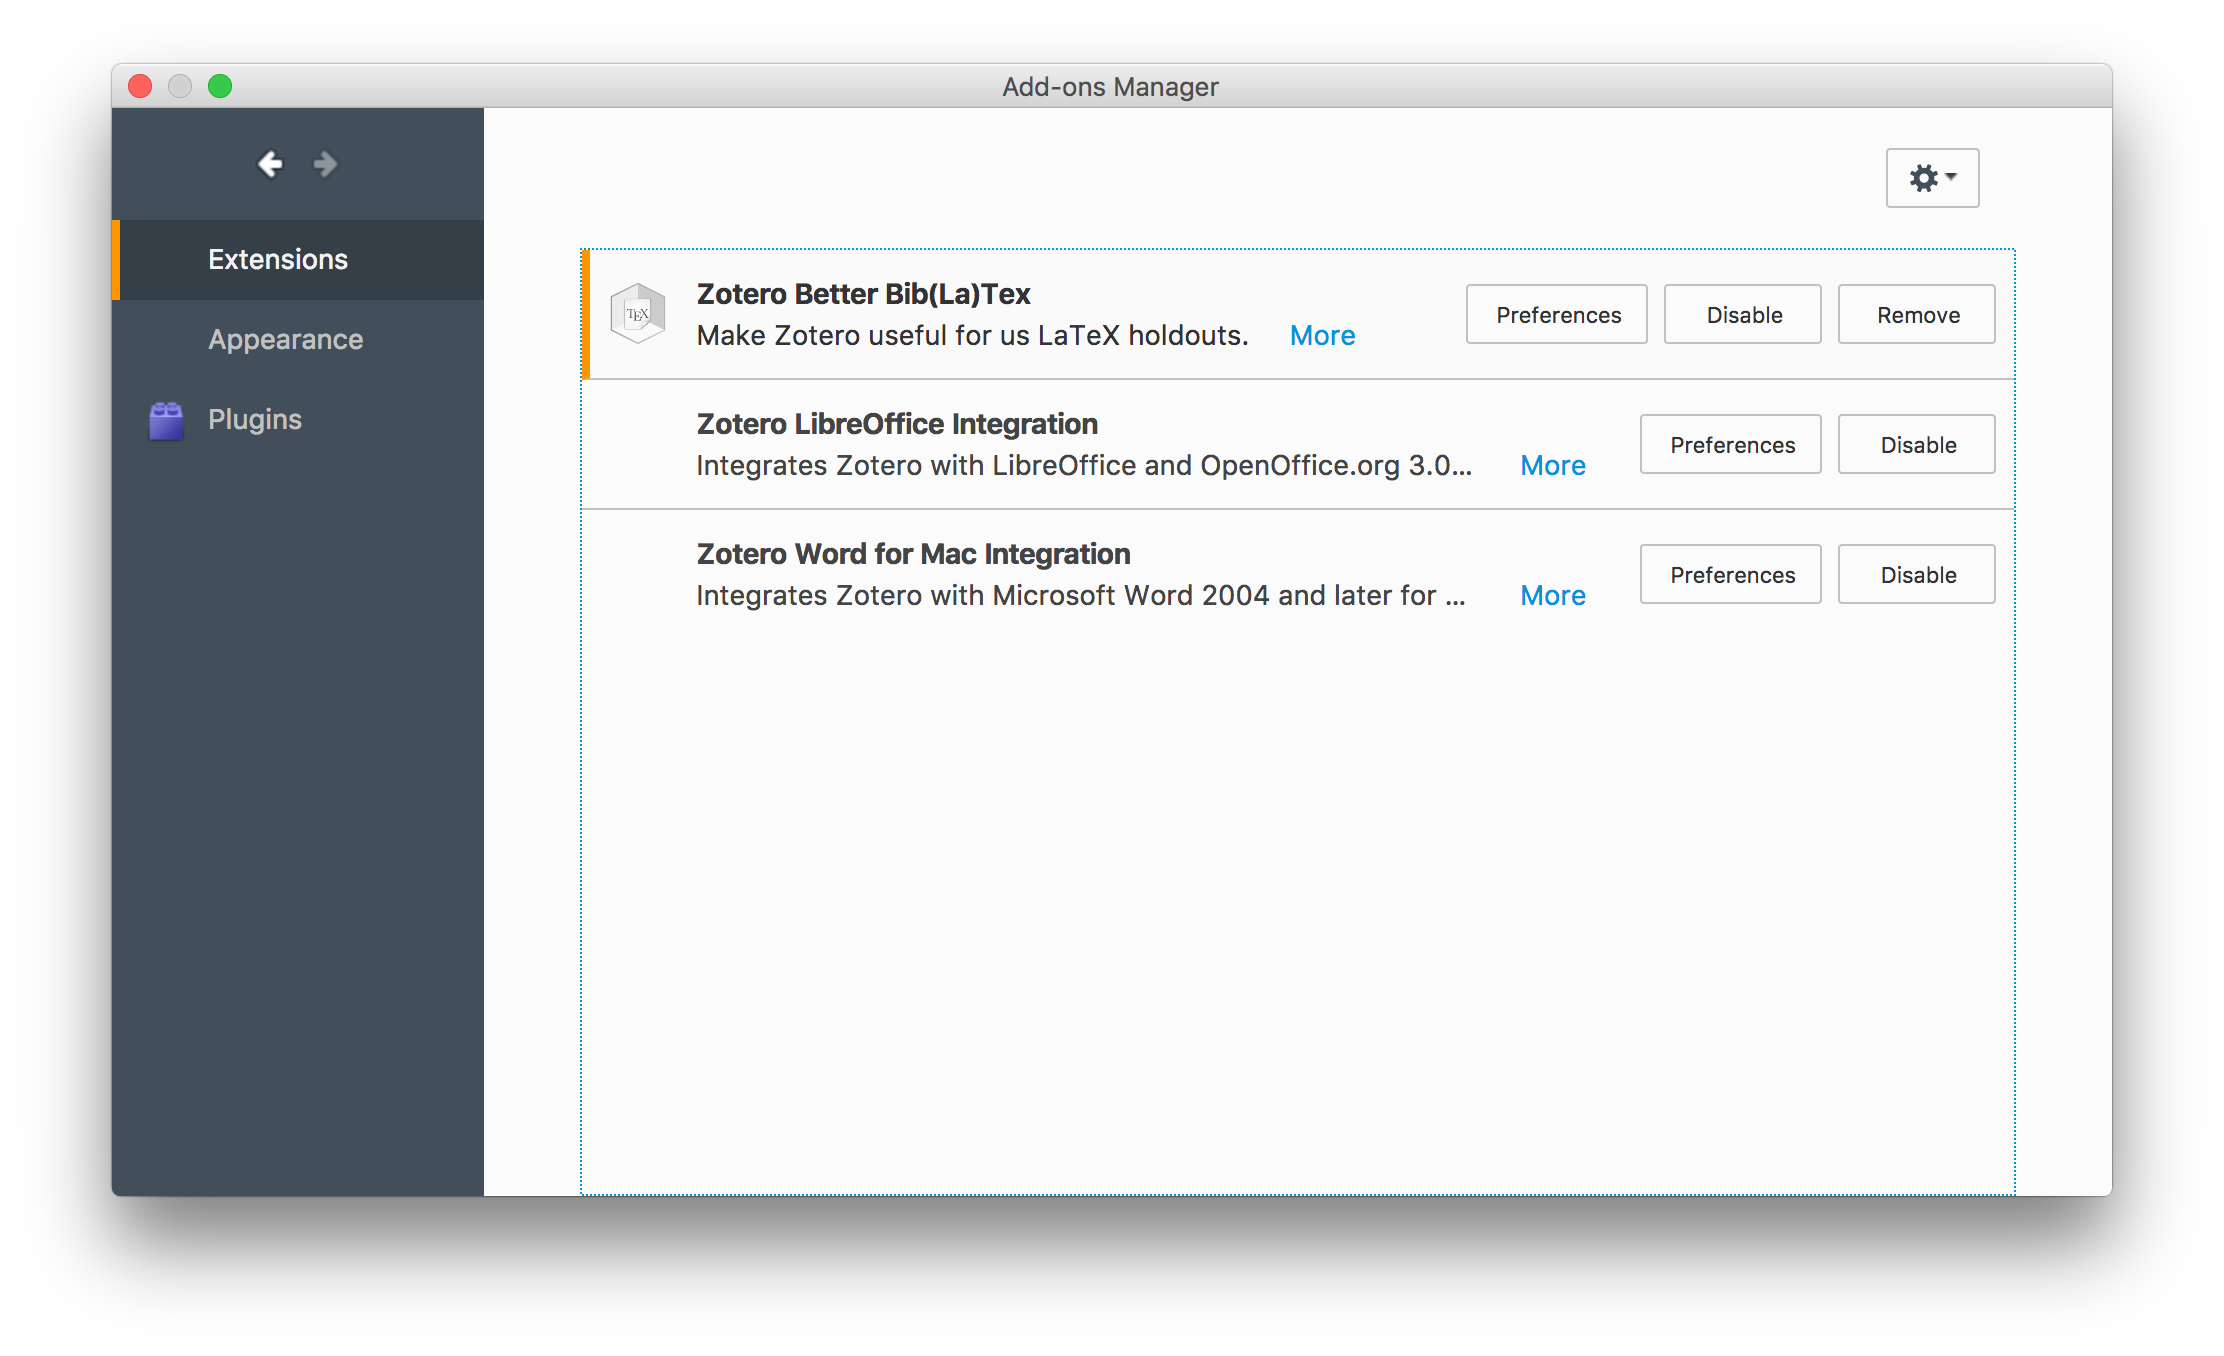
\includegraphics[width=\textwidth]{Figuras/plugins_zotero.png}
\caption{Installar Zotero y los plugins necesarios (especialmente el de flexbib).}
\label{etiqueta_figura1}
\end{center}
\end{figure}

\begin{figure}[!h]
\begin{center}
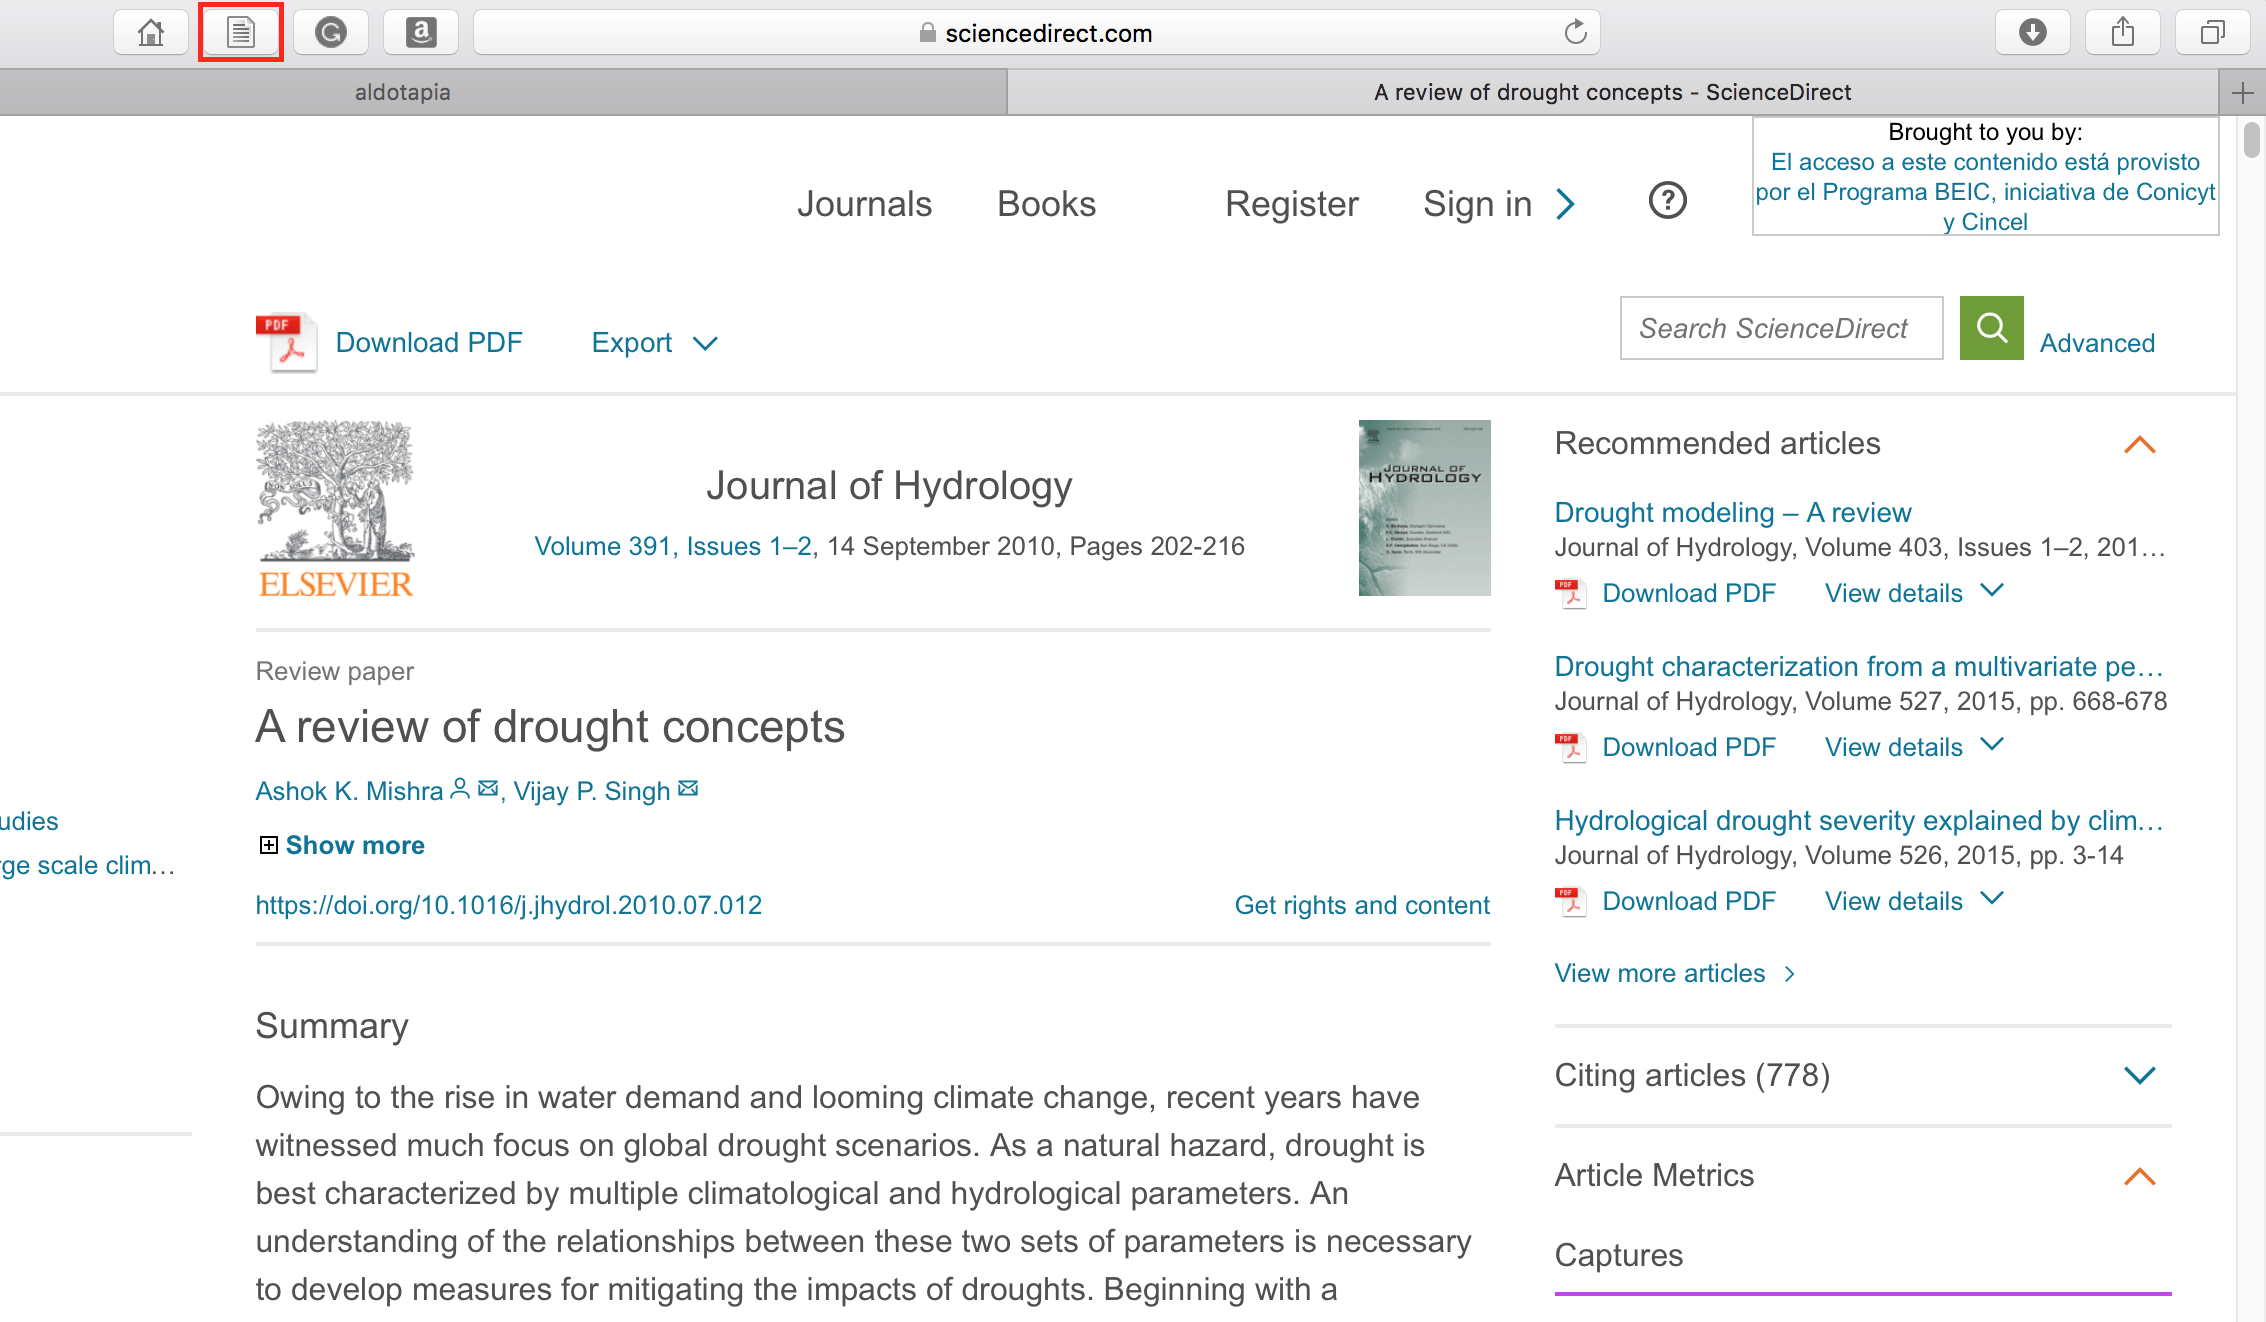
\includegraphics[width=\textwidth]{Figuras/zotero_web.png}
\caption{Clickear el ícono de Zotero para guardar cita}
\label{etiqueta_figura2}
\end{center}
\end{figure}

\begin{figure}[!h]
\begin{center}
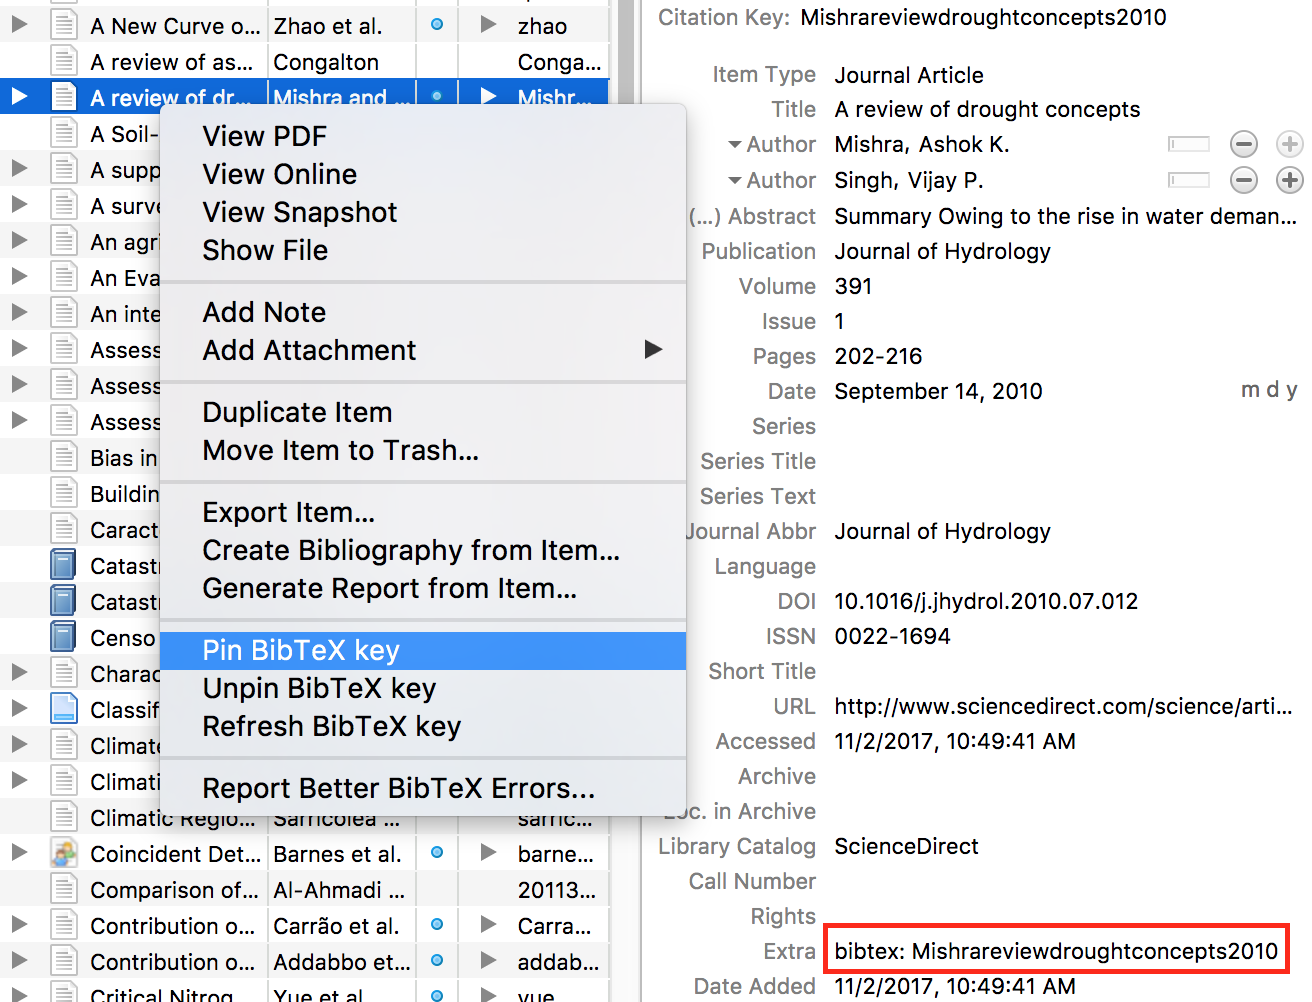
\includegraphics[width=\textwidth]{Figuras/zotero_pin.png}
\caption{Crear un pip de bibtex con la cita}
\label{etiqueta_figura3}
\end{center}
\end{figure}

\begin{figure}[!h]
\begin{center}
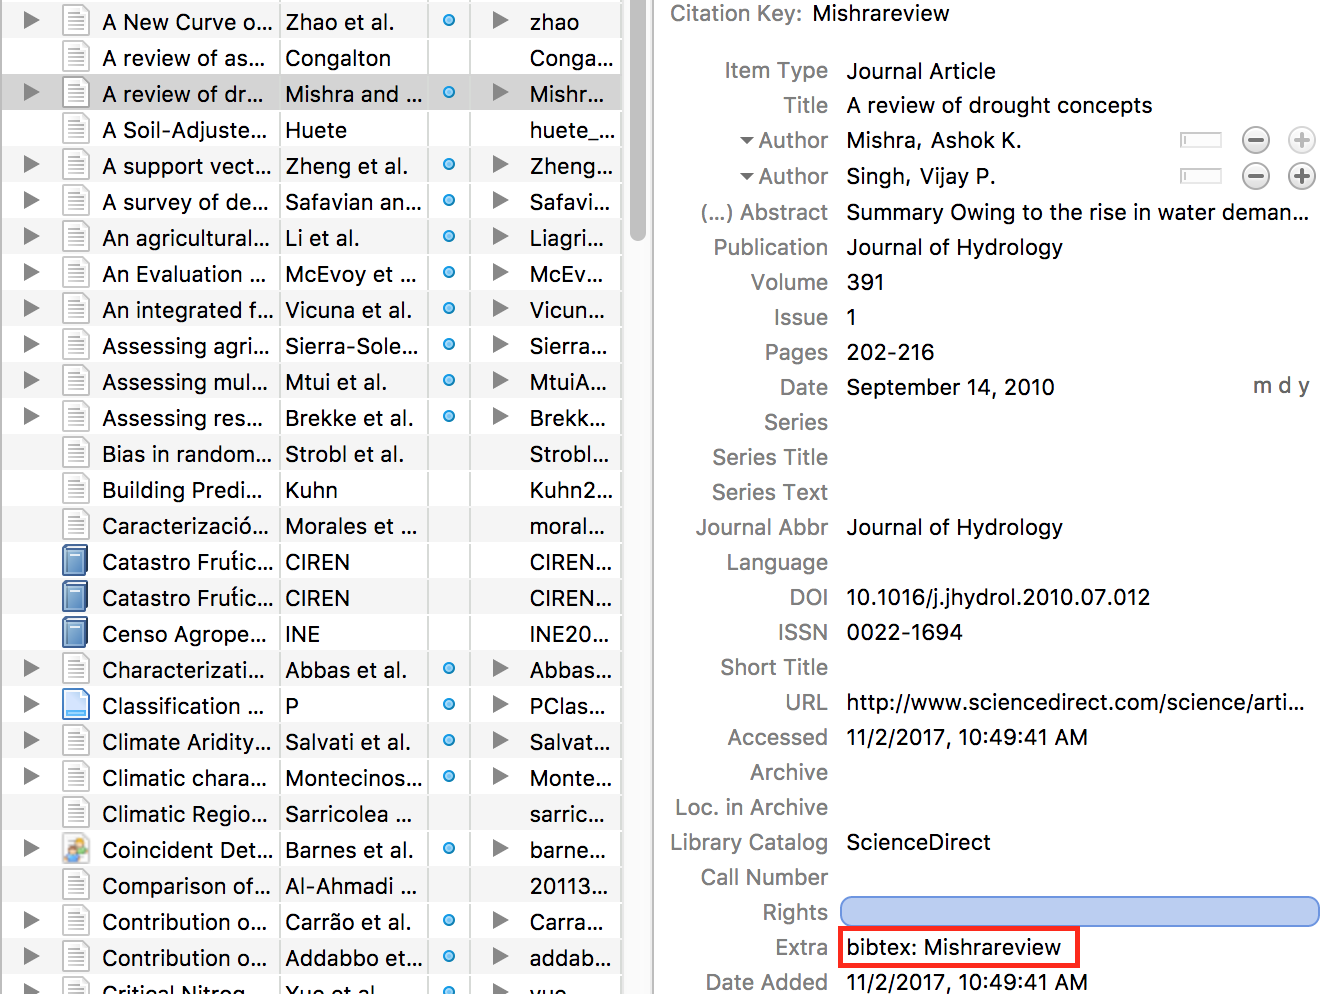
\includegraphics[width=\textwidth]{Figuras/zotero_pin2.png}
\caption{Modificar el pin si se requiere para facilitar la llamada en el documento}
\label{etiqueta_figura4}
\end{center}
\end{figure}

\begin{figure}[!h]
\begin{center}
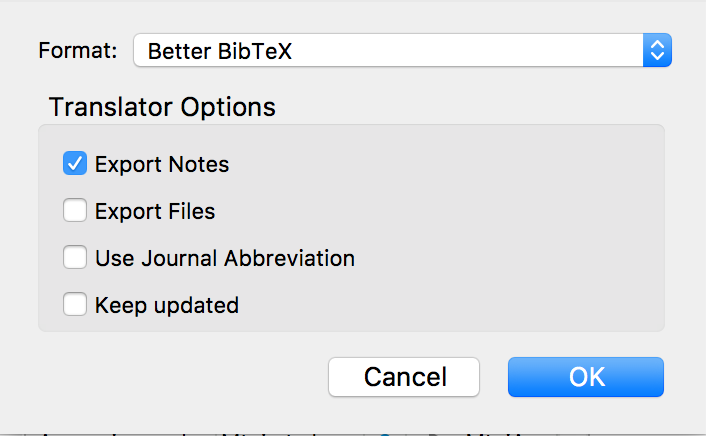
\includegraphics[width=\textwidth]{Figuras/better.png}
\caption{Exportar biblioteca como Better BibTex y guardarla en el mismo lugar donde está almacenado el archivo \texttt{nombre.tex}}
\label{etiqueta_figura5}
\end{center}
\end{figure}

\clearpage

Luego, llamar la cita en base al pin asignado, que en este caso es \verb!Mishrareview! con las funciones \verb!\cite{}! o \verb!\citep{}!. La primera es para citar con mención en el párrafo - como si \cite{Mishrareview} dijo algo - y la segunda; para citar con paréntesis \citep{Mishrareview}. Si se colocan comas entre los corchete para citar a una o más personas - como \verb!\citep{Mishrareview,huete1988}! - el resultado será una cita formateada con separadores \citep{Mishrareview,huete1988}.\\

\subsection{Información importante acerca de las citas\\}

XeLaTeX no compila la bibliografía automáticamente... La elección de este compilador es sólo por el uso de Century Gothic como fuente. Por lo tanto hay que compilar varias primero por XeLaTex, luego por BibTex (para crear la bibliografía), luego nuevamente por XeLaTex (aparecerá la bibliografía, pero las citas estarán con ?) y finalmente una última vez por XeLaTex y todo se compilará a la perfección. Para ello, he ocupado TeXShop para compilar.\\

\textbf{Información importante}: al utilizar RStudio para compilar los documentos, no es necesario seguir los pasos mencionados anteriormente. Sólo se utiliza el ícono \textit{Compile PDF} y el documento quedará correctamente compilado.

\section{Tablas\\}

Lo más sencillo para crear tablas es visitar el sitio web \href{https://www.tablesgenerator.com/latex_tables}{Tables Generator}. Sólo crean la tabla en excel, csv o otro formato. La cargan en el menu desplegable \verb!file! (Figura \ref{tabla1}) y copian el resultado que se obtiene (Figura \ref{tabla2}):

\begin{figure}[!h]
\begin{center}
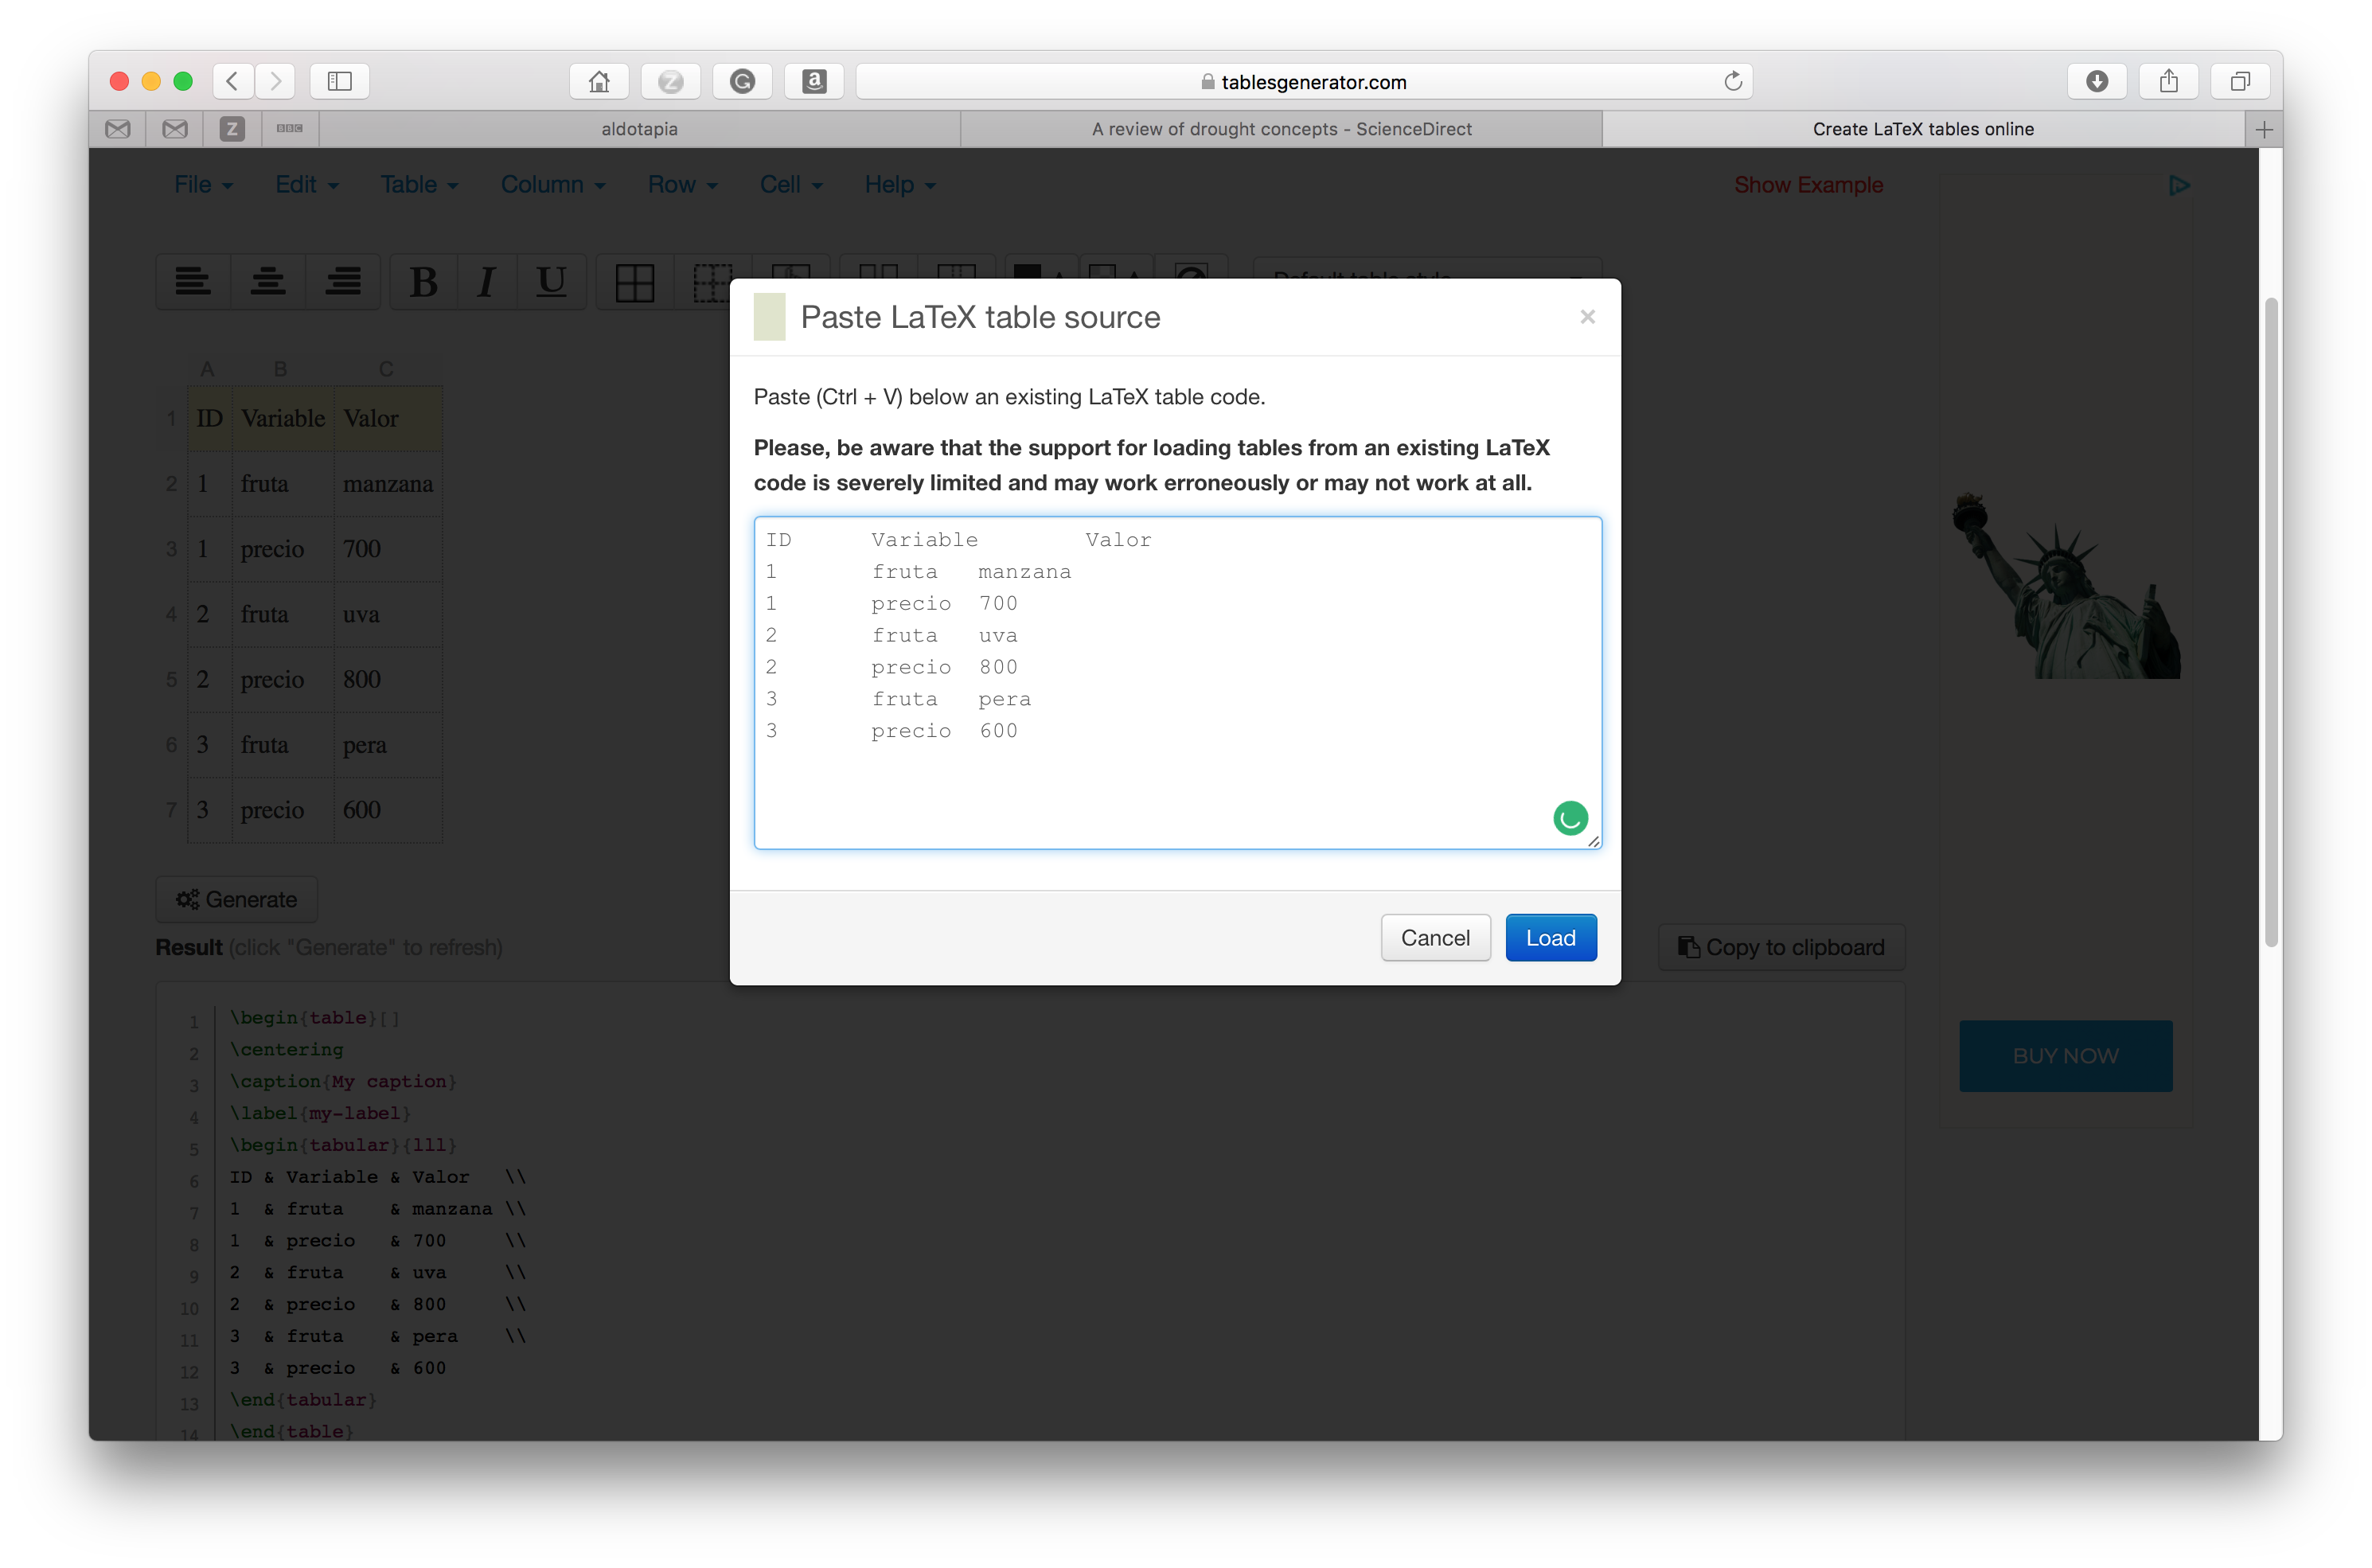
\includegraphics[width=\textwidth]{Figuras/tabla1.png}
\caption{Pegado de la tabla}
\label{tabla1}
\end{center}
\end{figure}

\begin{figure}[!h]
\begin{center}
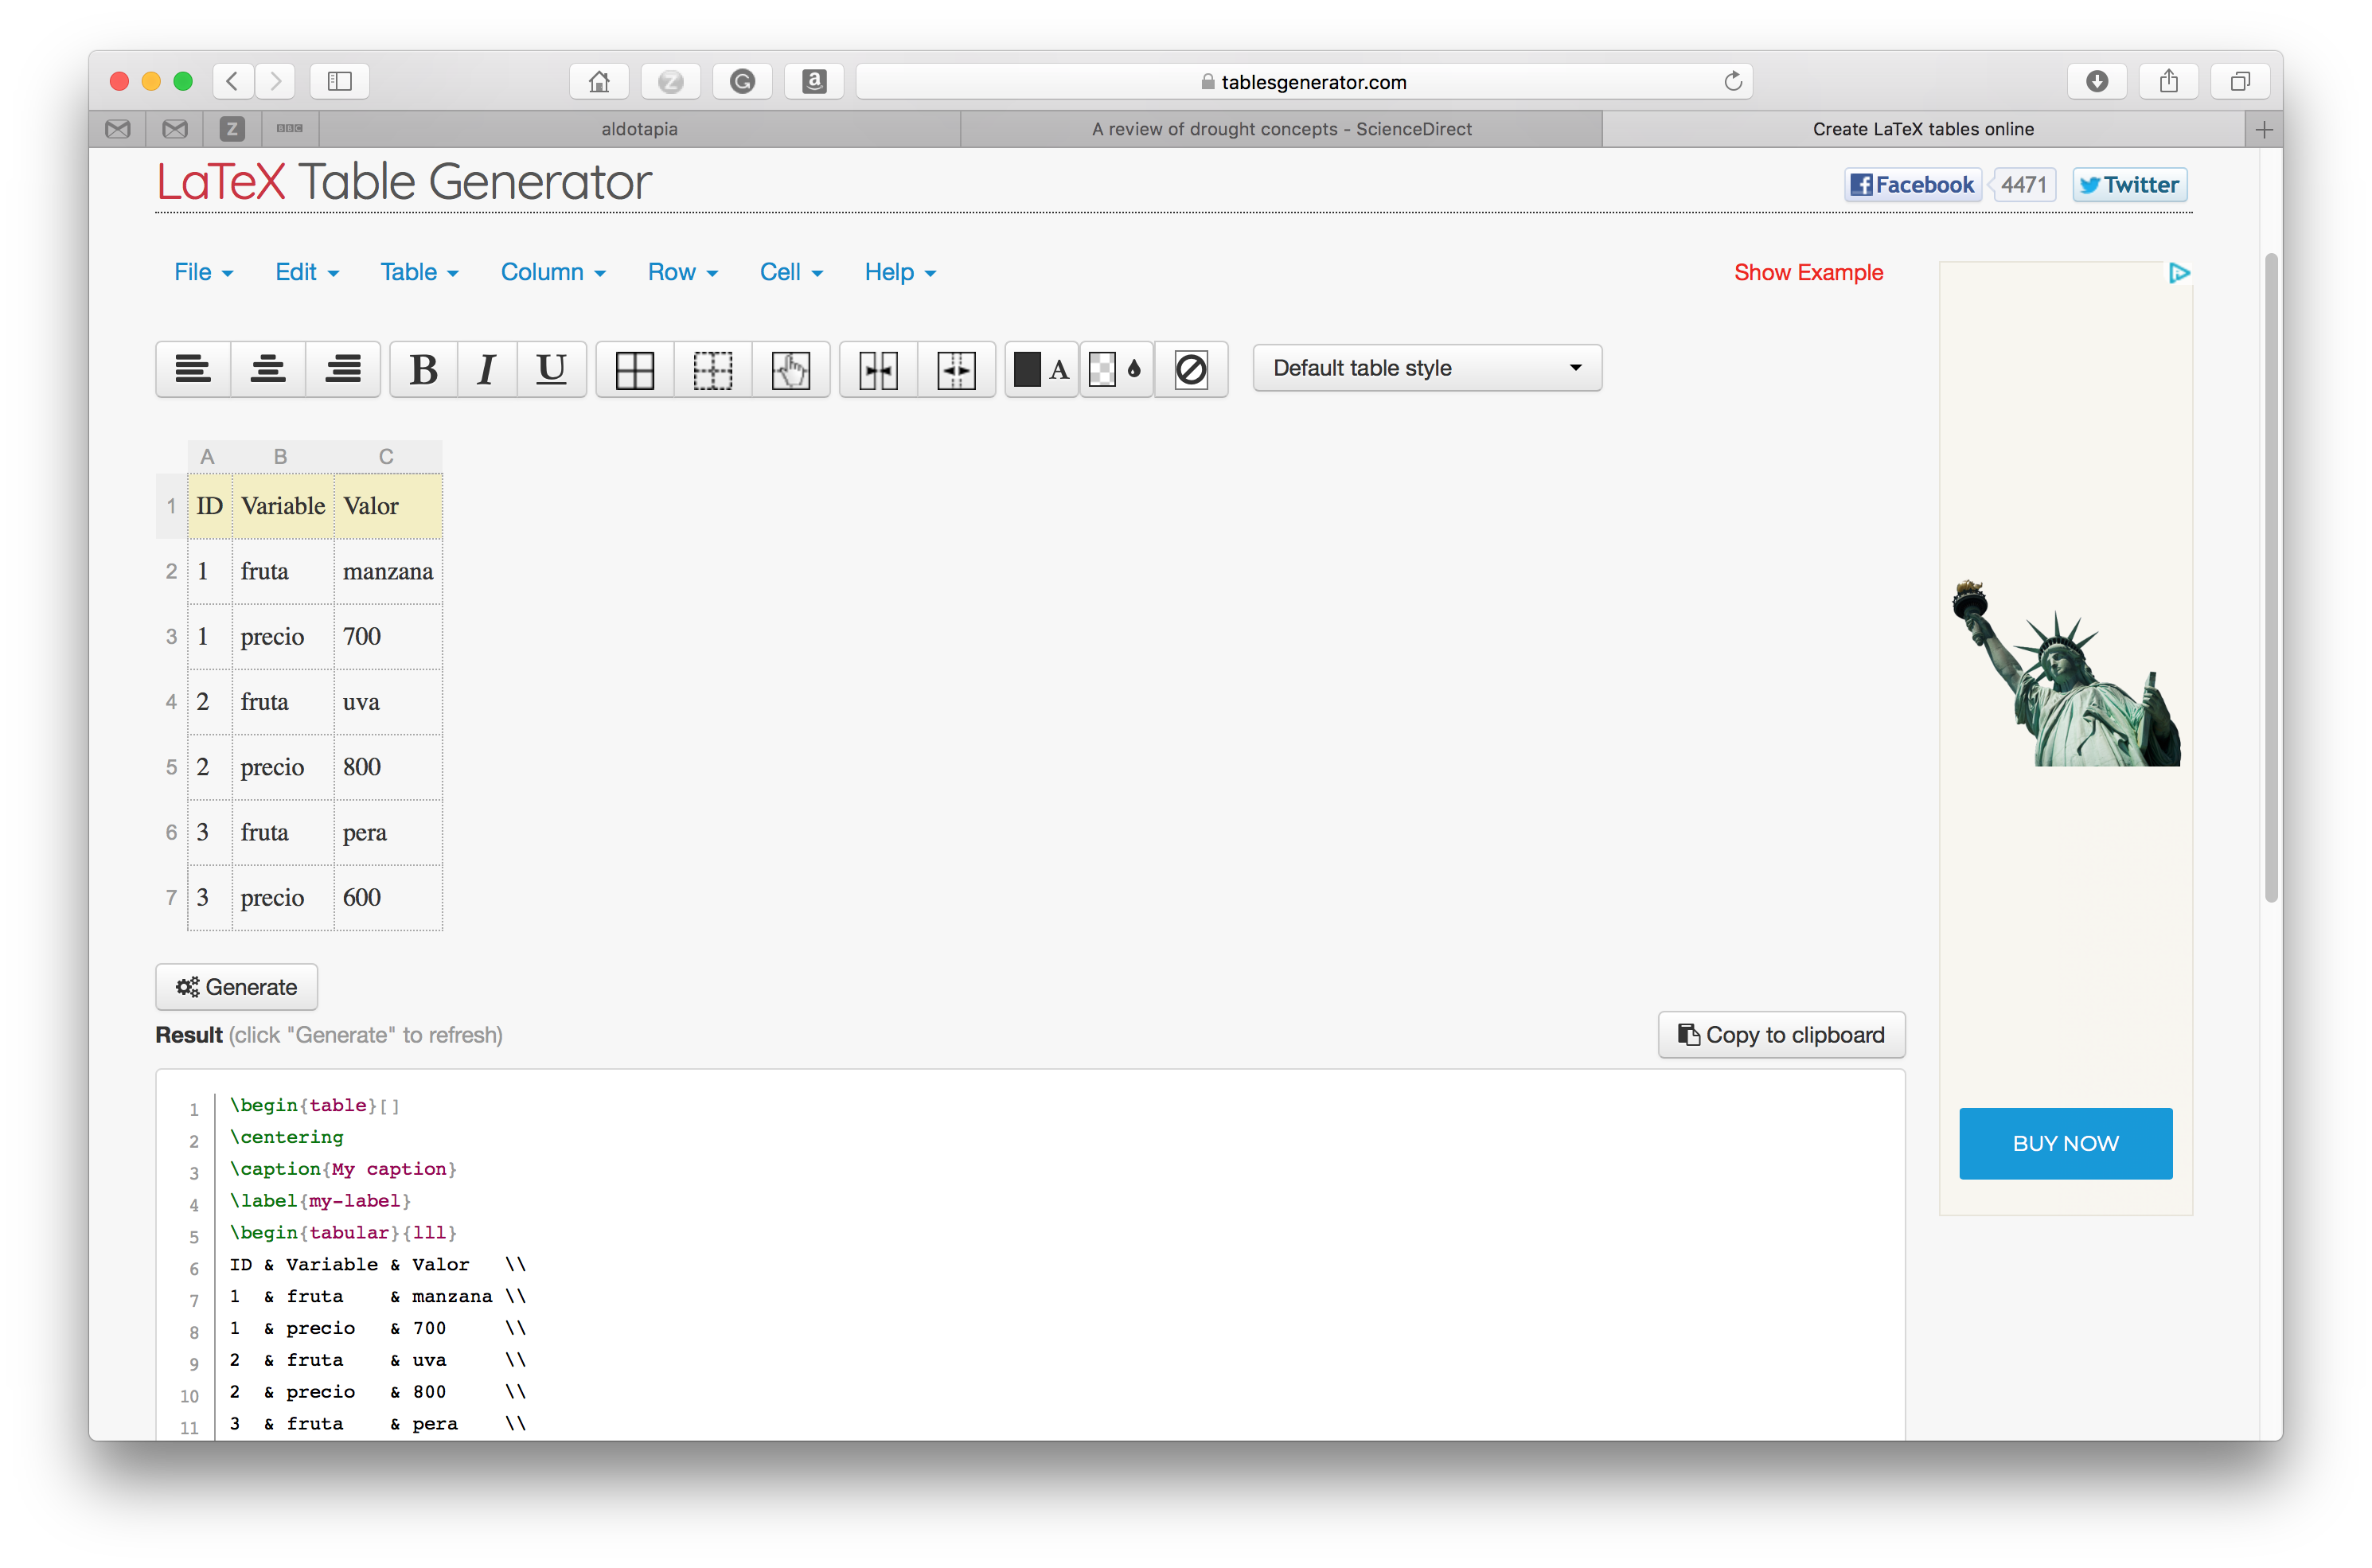
\includegraphics[width=\textwidth]{Figuras/tabla2.png}
\caption{Resultado}
\label{tabla2}
\end{center}
\end{figure}

\clearpage

\begin{table}[]
\centering
\caption{Descripción de la tabla}
\label{etiqueta_tabla}
\begin{tabular}{cll}
ID & Variable & Valor   \\
1  & fruta    & manzana \\
1  & precio   & 700     \\
2  & fruta    & uva     \\
2  & precio   & 800     \\
3  & fruta    & pera    \\
3  & precio   & 600    
\end{tabular}
\end{table}


\bibliographystyle{flexbib}
\bibliography{biblioteca.bib}


\end{document}  